\documentclass{../industrial-development}
%\documentclass[lecturenotes]{../industrial-development}
\graphicspath{{08-continious-integration/}}
\usepackage{color} %% это для отображения цвета в коде
\usepackage{listings}
\usepackage[utf8]{inputenx}
\usepackage{caption}
\DeclareCaptionFont{white}{\color{white}} %% это сделает текст заголовка белым
%% код ниже нарисует серую рамочку вокруг заголовка кода.
\DeclareCaptionFormat{listing}{\colorbox{gray}{\parbox{\textwidth}{#1#2#3}}}
\captionsetup[lstlisting]{format=listing,labelfont=white,textfont=white}
\title{Инструменты автоматической сборки и непрерывной интеграции в промышленной разработке}
\author{Харчев Дмитрий Михайлович, ИВТ-21 МО}
\date{}
\lstset{ %
	language=xml,                 % выбор языка для подсветки
	basicstyle=\tiny, % print whole listing small
	stringstyle=\color[rgb]{1,0.6,0.2},     % string literal style
	numberstyle=\color[rgb]{0.7,0.1,0.4}, % the style that is used for the line-numbers
	rulecolor=\color{black},         % if not set, the frame-color may be changed on line-breaks within not-black text (e.g. comments (green here))
	keywordstyle=\color[rgb]{0.18,0.28,0.75},       % keyword style
	commentstyle=\color[rgb]{0.4,0.4,0.4},    % comment style
	extendedchars=true,              % lets you use non-ASCII characters; for 8-bits encodings only, does not work with UTF-8
	%basicstyle=\small\sffamily, % размер и начертание шрифта для подсветки кода
	numbers=left,               % где поставить нумерацию строк (слева\справа)
	numberstyle=\tiny,           % размер шрифта для номеров строк
	stepnumber=1,                   % размер шага между двумя номерами строк
	numbersep=5pt,                % как далеко отстоят номера строк от подсвечиваемого кода
	backgroundcolor=\color{white}, % цвет фона подсветки - используем \usepackage{color}
	showspaces=false,            % показывать или нет пробелы специальными отступами
	showstringspaces=false,      % показывать или нет пробелы в строках
	showtabs=false,             % показывать или нет табуляцию в строках
	frame=single,              % рисовать рамку вокруг кода
	tabsize=2,                 % размер табуляции по умолчанию равен 2 пробелам
	captionpos=t,              % позиция заголовка вверху [t] или внизу [b] 
	breaklines=true,           % автоматически переносить строки (да\нет)
	breakatwhitespace=false, % переносить строки только если есть пробел
	escapeinside={\%*}{*)}   % если нужно добавить комментарии в коде
}
\begin{document}

\begin{frame}
  \titlepage
\end{frame}

\section{Автоматизация сборки}

\subsection{Определение}

\begin{frame} \frametitle{Автоматизация сборки}
	\begin{block}{Определение}
		Автоматизация сборки "--- этап написания скриптов или автоматизация широкого спектра задач, применяемого разработчиками в их повседневной деятельности. Включает в себя такие действия, как: 
	\end{block}
	
	\begin{itemize}
		\item Компиляция исходного кода в бинарный код 
		\item Сборка бинарного кода 
		\item Выполнение тестов 
		\item Разворачивание программы на производственной платформе 
		\item Написание сопроводительной документации или описание изменений новой версии 
	\end{itemize}
\end{frame}

\lecturenotes
Исторически так сложилось, что разработчики применяли автоматизацию сборки для вызова компиляторов и линковщиков из скрипта сборки, в отличие от вызова компилятора из командной строки. Довольно просто при помощи командной строки передать один исходный модуль компилятору, а затем и линковщику для создания конечного объекта. Однако, при попытке скомпилировать или слинковать множество модулей с исходным кодом, причём в определенном порядке, осуществление этого процесса вручную при помощи командной строки выглядит слишком неудобным. Гораздо более привлекательной альтернативой является скриптовый язык, поддерживаемый утилитой Make. Данный инструмент позволяет писать скрипты сборки, определяя порядок их вызова, этапы компиляции и линковки для сборки программы. GNU Make также предоставляет такие дополнительные возможности, как например, «зависимости» («makedepend»), которые позволяют указать условия подключения исходного кода на каждом этапе сборки. Это и стало началом автоматизации сборки. Основной целью была автоматизация вызовов компиляторов и линковщиков. По мере роста и усложнения процесса сборки разработчики начали добавлять действия до и после вызовов компиляторов, как например, проверку (check-out) версий копируемых объектов на тестовую систему. Термин «автоматизация сборки» уже включает в себя управление и действия до и после компиляции и линковки, так же как и действия при компиляции и линковке.

~\cite{Wiki_Build_automation}

\subsection{Задачи систем автоматической сборки в промышленной разработке}

\begin{frame} \frametitle{Задачи систем автоматической сборки в промышленной разработке}
 
  \begin{itemize}
  \item Улучшить качество продукта
  \item Ускорить процесс компиляции и линковки
  \item Избавить от излишних действий
  \item Минимизировать <<плохие (некорректные) сборки>>
  \item Вести истории сборок и релизов для разбора выпусков
  \item экономить время и деньги благодаря причинам, указанным выше
  \end{itemize}
\end{frame}

\lecturenotes
Продвинутая автоматизация сборки предоставляет возможность удаленному пользователю управлять обработкой распределённых сборок и/или распределённой обработкой сборки. Термин «распределённые сборки» подразумевает, что вызовы компилятора и линковщика могут передаваться множеству компьютеров для ускорения скорости сборки. Данный термин часто путают с «распределённой обработкой». Распределённая обработка означает, что каждый этап процесса может быть адресован разным машинам для выполнения ими данного шага. Например, этап после сборки может потребовать выполнения множества тестовых скриптов на множестве машин. Распределённая обработка позволяет послать команду на исполнение различных тестовых скриптов на разных машинах. Распределённая обработка — не то же самое, что и распределённая сборка! Распределённая обработка не может взять скрипты от make или maven, разбить их и послать команды на компиляцию и линковку различным машинам. Распределённый процесс сборки должен обладать определенной логикой, чтобы правильно определить зависимости в исходном коде для того чтобы выполнить этапы компиляции и линковки на разных машинах. Решение автоматизации сборки должно быть способно управлять этими зависимостями, чтобы выполнять распределённые сборки. Некоторые инструменты сборки могут распознавать подобные взаимосвязи автоматически (Rational ClearMake distributed, Electric Cloud ElectricAccelerator), а другие зависят от пользовательских указаний (Platform LSF lsmake) Автоматизация сборки, способная рассортировывать взаимосвязи зависимостей исходного кода, также может быть настроена на выполнение действий компиляции и линковки в режиме параллельного выполнения. Это означает, что компиляторы и линковщики могут быть вызваны в многопоточном режиме на машине, сконфигурированной с учётом наличия более одного процессорного ядра.

Не все инструменты автоматизации сборки могут выполнять распределённые сборки. Большинство из них лишь реализует поддержку распределённой обработки. Кроме того, большинство решений, поддерживающих распределённые сборки, могут лишь обрабатывать код на языках Си и C++. Решения автоматизации сборки, поддерживающие распределённую обработку, зачастую основаны на Make и не поддерживают Maven или Ant.

~\cite{Wiki_Build_automation}

\subsection{Обзор возможностей наиболее распространённых систем автоматической сборки}


\begin{frame} \frametitle{Make (1977 год)}
	\begin{block}{Определение}
		make "--- утилита предназначенная для автоматизации преобразования файлов из одной формы в другую. Правила преобразования задаются в скрипте с именем Makefile, который должен находиться в корне рабочей директории проекта.
	\end{block}	
\end{frame}
\lecturenotes
Сам скрипт состоит из набора правил, которые в свою очередь описываются:
 Целями (то, что данное правило делает)
 Реквизитами (то, что необходимо для выполнения правила и получения целей)
 Командами (выполняющими данные преобразования)
~\cite{Habr_make}

\begin{frame}[fragile] \frametitle{Make}
\begin{lstlisting}[label=some-code,caption=Синтаксис makefile в общем виде]
<objectives>: <requisites>
	<comand #1>
	...
	<comand #n>

\end{lstlisting}

\end{frame}
\lecturenotes
Индентация осуществляется исключительно при помощи символов табуляции, каждой команде должен предшествовать отступ.
Правило make это ответы на три вопроса:
{Из чего делаем? (реквизиты)} ---> [Как делаем? (команды)] ---> {Что делаем? (цели)}

\begin{frame}[fragile] \frametitle{Make}
\begin{lstlisting}[label=some-code,caption=Простейший Makefile]
hello: main.c
	gcc -o hello main.c
\end{lstlisting}
\begin{lstlisting}[label=some-code,caption=Команда для компиляции]
$ make <objective>
\end{lstlisting}

\end{frame}
\lecturenotes
Данный Makefile состоит из одного правила, которое в свою очередь состоит из цели — «hello», реквизита — «main.c», и команды — «gcc -o hello main.c». Теперь, для компиляции достаточно дать команду make в рабочем каталоге. По умолчанию make станет выполнять самое первое правило, если цель выполнения не была явно указана при вызове:

\begin{frame}[fragile] \frametitle{Make}
	\begin{lstlisting}[label=some-code,caption=Пример makefile]
	TARGET = hello
	PREFIX = /usr/local/bin
	.PHONY: all clean install uninstall
	all: $(TARGET)
	clean:
		rm -rf $(TARGET) *.o
	main.o: main.c
		gcc -c -o main.o main.c
	hello.o: hello.c
		gcc -c -o hello.o hello.c
	$(TARGET): main.o hello.o
		gcc -o $(TARGET) main.o hello.o
	install:
		install $(TARGET) $(PREFIX)
	uninstall:
		rm -rf $(PREFIX)/$(TARGET)
	
	\end{lstlisting}
\end{frame}

\lecturenotes
Командой make производят компиляцию программы, командой make install — установку. Такой подход весьма удобен, поскольку все необходимое для сборки и развертывания приложения в целевой системе включено в один файл (забудем на время о скрипте configure). Обратите внимание на то, что в первом случае мы не указываем цель, а во втором целью является вовсе не создание файла install, а процесс установки приложения в систему. Проделывать такие фокусы нам позволяют так называемые фиктивные (phony) цели. Вот краткий список стандартных целей:
all — является стандартной целью по умолчанию. При вызове make ее можно явно не указывать.
clean — очистить каталог от всех файлов полученных в результате компиляции.
install — произвести инсталляцию
uninstall — и деинсталляцию соответственно.

Для того чтобы make не искал файлы с такими именами, их следует определить в Makefile, при помощи директивы .PHONY. Далее показан пример Makefile с целями all, clean, install и uninstall и использующий две переменные: TARGET — для определения имени целевой программы и PREFIX — для определения пути установки программы в систему.
~\cite{Yandex_Build_Automation}

\begin{frame} \frametitle{Make}
	\begin{block}{Примущества}
		\begin{itemize}
			\item Единый формат описания процесса сборки
		\end{itemize}
	\end{block}
\end{frame}

\lecturenotes
Основное преимущество состоит в том, что Make определяет единый формат описания
сборки, то есть мы всегда знаем, что есть команды определяющие стадию, а то, что написано через табуляцию это название команд.
~\cite{Yandex_Build_Automation}

\begin{frame} \frametitle{Make}
	\begin{block}{Недостатки}
	\begin{itemize}
		\item Платформозависим
		\item Tab символы в Makefile
		\item Нет поддержки Java задач, параметров,
		плагинов
	\end{itemize}
	\end{block}
\end{frame}

\lecturenotes
Недостатки тоже достаточно очевидны, во-первых, так как внутри make файла находятся команды операционной системы, такой билд все равно будет платформозависимым. Например, сейчас многие проекты, написанные на C или C++, попрежнему собираются make файлами и там делаются различные ветвления, условная логика для того, чтобы такой билд был переносимым.
Кроме того, в make файлах используется табуляция (команды от названия стадий отделяются табуляцией). Табуляции в текстовых редакторах по-умолчанию не видны, поэтому если при редактировании в ненужное место попадет пробел, то такой файл будет неправильным.
~\cite{Yandex_Build_Automation}

\begin{frame} \frametitle{Apache Ant (2000 год)}
	\begin{block}{Определение}
		Apache Ant (<<Another Neat Tool>>) "--- утилита для автоматизации процесса сборки программного продукта. Является платформонезависимым аналогом утилиты make, где все команды записываются в XML-формате
	\end{block}
\end{frame}

\lecturenotes
Первым инструментом, который был разработан на Java и для Java был Apache Ant, был разработан в 2000 году.
~\cite{Wiki_Apache_Ant}
~\cite{Yandex_Build_Automation}

\begin{frame}[fragile] \frametitle{Apache Ant}
	\begin{lstlisting}[label=some-code,caption=build.xml]
	<?xml version="1.0"?>
	<project default="build" basedir=".">
		<property name="name" value="AntBuildJar"/>
		<property name="src.dir" location="${basedir}/src"/>
		<property name="build" location="${basedir}/build"/>
		<property name="build.classes" location="${build}/classes"/>
		<path id="libs.dir">
		<fileset dir="lib" includes="**/*.jar"/>
		</path>
		<target name="build" depends="clean" description="Builds the application">
			<mkdir dir="${build.classes}"/>
			<javac srcdir="${src.dir}"
					destdir="${build.classes}"
					debug="false"
					deprecation="true"
					optimize="true" >
				<classpath refid="libs.dir"/>
			</javac>
			<copy todir="${build.classes}">
				<fileset dir="${src.dir}" includes="**/*.*" excludes="**/*.java"/>
			</copy>
			<jar jarfile="${build}/${name}.jar">
				<fileset dir="${build.classes}"/>
			</jar>
		</target>	
		<target name="clean" description="Removes all temporary files">
			<delete dir="${build.classes}"/>
		</target>
	</project>
	\end{lstlisting}
\end{frame}
\lecturenotes
Конфигурационный файл build.xml показан на слайде. В нем содержатся описание названий стадий, зависимости стадий друг от друга.
<target name="build" - стадия билда проекта. Внутри этой стадии происходит создание директорий, компилирование исходного кода, копирование необходимых файлов и создание JAR-файла.
<target name="clean" - стадия очистки проекта.
Кроме того, они могут содержать некоторые java специфичные вещи.Здесь, например, в секции javac это конфигурациия сборки java кода, различные опции вроде classpath и так далее. Команда, которая запускает компиляцию ant <название цели>. Например: ant compile, ant clean или ant clean compile.
~\cite{Yandex_Build_Automation}

\begin{frame} \frametitle{Apache Ant}
	\begin{block}{Преимущества}
	\begin{itemize}
		\item Поддержка Java-специфичных задач
		\item Переносимость между платформами
		\item Возможность расширения (плагины)
		\item Параметризованные билды
	\end{itemize}
	\end{block}
\end{frame}
\lecturenotes
Поскольку конфигурация билда идет в xml, явно никакие консольные команды операционной системы не используются, поэтому такой билд будет переносимым между платформами. Кроме того, Ant это первая система, которая добавила возможность писать расширения (плагины). Очень большая часть функциональности Ant'а реализована через плагины. Например, для того, чтобы запускать тесты в JUnit существует плагин. Также Ant позволяет запускать параметризованные билды, то есть в отдельной секции можно хранить отдельные параметры, например, версии используемых библиотек и позднее замена версий будет означать замену библиотек в проекте
~\cite{Yandex_Build_Automation}

\begin{frame} \frametitle{Apache Ant}
	\begin{block}{Недостатки}
		\begin{itemize}
			\item Нет конвенций версионирования кода
			\item Нет конвенций по расположению кода
			\item Нет автоматического управления
			зависимостями (их кладут в lib/)
			\item Произвольный набор целей (нет жизненного
			цикла)
			\item Императивный стиль описания билда
			(последовательность действий)
			\item Не поддерживает JUnit 4
		\end{itemize}
	\end{block}	
\end{frame}
\lecturenotes
Ant имеет ряд недостатков:
Ant никак не определяет конвенции версионирования кода.
Нет конвенций по расположению кода, то есть открыв проект на Ant'е код может лежать где угодно, естественно, что чаще всего его кладут в одну и ту же папку, но это никак не гарантируется самим Ant.
Самый главный недостаток Apache Ant, что в нем нет управления зависимостями. Все зависимости идут вместе с проектом (как правило в папке /lib). В больших проектах обычно библиотек много.
Ant совершенно не определяет какого то набора целей, цели можно называть как угодно и из-за этого приходится разбираться какая цель что делает, то есть нет жизненного цикла у билда.
Как и все предыдущие инструменты Ant подходит к описанию билды императивно, то есть билд состоит из последовательности действий, которые нужно выполнить, чтобы собрать проект.
С точки зрения тестирования Ant имеет еще один недостаток, Ant не поддерживает JUnit 4, наиболее популярный тестовый фреймворк.
~\cite{Yandex_Build_Automation}

\begin{frame} \frametitle{Apache Maven (2004 год)}
	\begin{block}{Определение}
		Apache Maven "--- фреймворк для автоматизации сборки проектов на основе описания их структуры в файлах на языке POM(Project Object Model), являющемся подмножеством XML
	\end{block}
\end{frame}
\lecturenotes
Следующим инструментом, который пришел на замену Apache Ant стал Apache Ivy. Он появился в 2004 году и также использует файл конфигурации на xml pom.xml, название файла является аббревеатурой Project Object Model, то есть объектная модель проекта.

~\cite{Wiki_Apache_Ant}
~\cite{Yandex_Build_Automation}


\begin{frame}[fragile] \frametitle{Apache Maven}
	\begin{lstlisting}[label=some-code,caption=pom.xml]
	<project>
		<modelVersion>4.0.0</modelVersion>
		<groupId>com.mycompany.app</groupId>
		<artifactId>my-app</artifactId>
		<version>1.0</version>
			<dependencies>
				<dependency>
					<groupId>junit</groupId>
					<artifactId>junit</artifactId>
					<version>3.8.1</version>
					<scope>test</scope>
				</dependency>
			</dependencies>
	</project>
	\end{lstlisting}
\end{frame}
\lecturenotes
На слайде представлен пример конфигурационного файла pom.xml.
В первой строке указывается версия модели для POM-ов Maven 2.x всегда 4.0.0.
Далее идут координаты проекта, то есть набор значений, который
позволяет однозначно идентифицировать этот проект. Затем перечисляются зависимости от библиотек. После координаты необходимой библиотеки на примере JUnit и указывается, что эта библиотека используется только для запуска и компилирования тестов.
~\cite{Yandex_Build_Automation}

\begin{frame} \frametitle{Apache Maven}
	\begin{block}{Преимущества}
		\begin{itemize}
			\item Конвенции расположения кода, тестов,
			ресурсов и т.д.
			\item Четкий жизненный цикл: цели предопределены
			\item Способ поделиться кодом с другими "---
			удаленные репозитории зависимостей
			\item Понятный механизм хранения зависимостей~---локальный репозиторий
		\end{itemize}
	\end{block}	
\end{frame}
\lecturenotes
Apache Maven принес с собой много преимуществ. Во-первых, Maven внес четкие правила расположения кода, то есть исходные коды продукта лежат в одной директории, исходные коды тестов в другой директории, ресурсы/конфигурационные файлы в третьей и так далее. В связи с этим в проекте легко ориентироваться.
Maven использует набор предопределенных целей для выполнения основных задач, то есть есть цель для компиляции, тестирования, создания отчетов и так далее. Хотя есть возможность создавать свои цели.
Maven имеет способ поделиться кодом с другими участниками разработки, вводя такое понятие, как удаленный репозиторий - сервера на которые закачиваются готовые пакеты с скомпилированным кодом, исходными кодами, документацией и другие учатники разработки могут их забрать.
Следующее преимущество это понятный механизм хранения зависимостей - локальный репозиторий это каталог в файловой системе, в котором сохраняются копии скомпилированных бинарных файлов, документация и так далее. По сути это копия удаленного репозитория.
~\cite{Yandex_Build_Automation}

\begin{frame} \frametitle{Apache Maven}
	\begin{block}{Преимущества}
		\begin{itemize}
			\item Правила версионирования кода
			\item Поддержка многомодульных проектов
			\item Декларативный подход к описанию билда
			\item Модульная структура (даже простые действия
			делают плагины)
		\end{itemize}
	\end{block}	
\end{frame}
\lecturenotes
Кроме того, Maven вводит четкие правила версионирования кода, вводят понятия релизов (release) и снепшотов (snapshot) и как версии должны меняться одна к другой.
Maven это первая система, которая поддерживает многомодульные проекты. Это значит, что можно разбивать проект на небольшие кусочки - модули, которые могут собираться по отдельности, распространяться, передаваться, в общем версионироваться по отдельности, это очень удобно.
Maven это первая система, которая описывает подход декларативно, не в какой последовательности нужно выполнить шаги, а что мы хотим получить на выходе.
Ну и последнее это поддержка плагинов (модульная структура). Даже простые действия делают плагины: есть плагин для компиляции, тестирования, создания отчётов.
~\cite{Yandex_Build_Automation}

\begin{frame} \frametitle{Gradle}
	\begin{block}{Определение}
		Gradle "--- система автоматической сборки, построенная на принципах Apache Ant и Apache Maven, но предоставляющая DSL(Domain-specific language, DSL "--- <<язык, специфический для предметной области>>) на языке Groovy вместо традиционной XML-образной формы представления конфигурации проекта.
	\end{block}
\end{frame}

\lecturenotes
	Написан на Groove в 2009 году
	В отличие от Apache Maven, основанного на концепции жизненного цикла проекта, и Apache Ant, в котором порядок выполнения задач (targets) определяется отношениями зависимости (depends-on), Gradle использует направленный ациклический граф для определения порядка выполнения задач.
	Gradle был разработан для расширяемых многопроектных сборок, и поддерживает инкрементные сборки, определяя, какие компоненты дерева сборки не изменились и какие задачи, зависимые от этих частей, не требуют перезапуска.
	Основные плагины предназначены для разработки и развертывания Java, Groovy и Scala приложений, но готовятся плагины и для других языков программирования.
~\cite{Wiki_Gradle}
~\cite{Yandex_Build_Automation}
	
\begin{frame}[fragile] \frametitle{Gradle}
	\begin{lstlisting}[label=some-code,caption=build.gradle]
		apply plugin: 'java'
		apply plugin: 'application'
		mainClassName = 'hello.HelloWorld'

		repositories {
		mavenLocal()
		mavenCentral()
		}

		jar {
		baseName = 'gs-gradle'
		version =  '0.1.0'
		}

		dependencies {
		}
		

		task wrapper(type: Wrapper) {
		gradleVersion = '1.11'
		}
	\end{lstlisting}
\end{frame}
\lecturenotes
На слайде показан пример конфигурационного файла build.gradle для приложения HelloWorld.
В первых строках файла указываются используемые плагины и название мейн класса приложения. Затем раздел используемых репозиториев. Далее указано название и версия JAR-файла. Раздел зависимостей в данном случае пуст из-за того, что приложение простое.
Теперь остановимся подробней на задаче wrapper. Эта очень полезная задача, наверное, самое гениальное решение, призванное облегчить жизнь программистам. Выполнив 
gradle wrapper 
получим следующий результат: скрипт создал нам исполняемые файлы gradlew для *nix, gradlew.bat для Windows, а также папки gradle и .gradle. Скрытую папку .gradle можно не включать в репозиторий, там содержатся библиотеки зависимостей. Все основное лежит в gradle и в самом файле gradlew. Теперь мы смело может отдавать наш проект любому человеку, имеющему jdk нужной версии, и он самостоятельно сможет скомпилировать, собрать, установить проект, используя ./gradlew. 
~\cite{Habr_Gradle}
~\cite{Yandex_Build_Automation}

\begin{frame} \frametitle{Gradle}
	\begin{block}{Преимущества}
		\begin{itemize}
			\item Поддерживает основные возможности Maven
			\item Файл build.gradle с DSL на Groovy
			\item Инкрементная компиляция
			\item Использует те же удаленные репозитории, что
			и Maven
			\item Эмулирует поведение Maven, но можно
			задавать свой порядок целей
			\item Поддерживает плагины, несовместимые с
			Maven
		\end{itemize}
	\end{block}		
\end{frame}
\lecturenotes
Gradle умеет все тоже самое, что и Maven.
Gradle использует в качестве файла конфцигурации DSL(Domain-specific language) предметно-ориентированный язык на Groove.
Основная фишка Gradle по сравнению с Maven это поддержка инкрементальной компиляции, то есть Gradle умеет собирать только те исходные коды, которые изменились, для больших проектов это сильно ускоряет разработку.
В остальном Gradle очень похож на Maven, использует те же удаленные репозитории, имеет такой же набор предопределенных целей, но можно задавать и свои.
Ну и также может расширяться с помощью плагинов, которые, к сожалению, не совместмы с Maven.
~\cite{Yandex_Build_Automation}

\section {Непрерывная интеграция}
\subsection {Понятие непрерывной интеграции}

\begin{frame} \frametitle{Непрерывная интеграция}
		итерационные сборки $\Rightarrow$  ночные сборки $\Rightarrow$  непрерывная сборка
	\end{frame}
\lecturenotes
Термин Continuous Integration введен Мартином Фаулером (Martin Fowler) и Кентом Беком (Kent Beck). Данный термин был придуман ими для обозначения практики частой сборки (интеграции) проекта. Максимально частая сборка является логичным продолжением цепочки представленной на слайде.
В настоящее время Continuous Integration (непрерывная интеграция) одна из практик применяемых в семействе гибких (Agile) методологий. В подобных методологиях она удачно сочетается с другими практиками, такими как модульное(unit) тестирование, рефакторинг, стандарт кодирования. Но даже без них можно получить пользу от непрерывной интеграции.
~\cite{Custis_Continuous Integration}

\subsection {Принципы непрерывной интеграции}

\begin{frame} \frametitle{Принципы}
	\begin{block}{На выделенном сервере организуется служба, в задачи которой входят:}
		\begin{itemize}
			\item Получение исходного кода из репозитория
			\item Сборка проекта
			\item Выполнение тестов
			\item Развёртывание готового проекта
			\item Отправка отчетов
		\end{itemize}
	\end{block}
	\begin{block}{Локальная сборка может осуществляться:}
		\begin{itemize}
		\item По внешнему запросу
		\item По расписанию
		\item По факту обновления репозитория и по другим критериям
		\end{itemize}
	\end{block}
\end{frame}
\lecturenotes
~\cite{Custis_Continuous Integration}

\subsection {Достоинства}

\begin{frame} \frametitle{Достоинства}
	\begin{block}{}
			\begin{itemize}
			\item Проблемы интеграции выявляются и исправляются быстро,
			что оказывается дешевле
			\item Немедленный прогон модульных тестов для свежих
			изменений
			\item Постоянное наличие текущей стабильной версии вместе с
			продуктами сборок "--- для тестирования, демонстрации, и т.~п.
			\item Немедленный эффект от неполного или неработающего
			кода приучает разработчиков к работе в итерактивном
			режиме с более коротким циклом
		\end{itemize}
	\end{block}
\end{frame}

\lecturenotes
Скорейшее обнаружение ошибок (в течение суток или нескольких часов после коммита) делает процесс их устранения очень быстрым и «дешевым». Обычно болезненный процесс интеграции перестает растягиваться на месяца и становиться кошмаром программистов.

Все анализаторы кода и тесты, которые вы используете и написали, обязательно запускаются над каждой сборкой. Если в систему контроля версий попал «плохой» код — вы об этом узнаете. И не важно, нарушен ли один из стандартов кодирования, или статический анализатор кода показывает, что в код попала потенциальная ошибка или тесты не прошли, а может просто покрытие кода модульными тестами упало ниже необходимого минимума. Вы об этом узнаете и сможете принять меры.
Более того, запуск всех этих анализаторов полезен не только для определения состояния в текущий момент времени, но и для анализа тенденций. Можно увидеть, когда ваш код стал сильно больше, сложнее, в каких модулях эта сложность сконцентрирована. Да, это требует наличия и использования соответствующего инструментария.
Чем больше и серьезней проведена работа по настройке сервера интеграции, тем больше пользы можно получить. Если ваш сервер просто собирает проект после каждого изменения в коде, то польза от него не так велика, но и усилий на него почти не потрачено.

На руках есть работоспособная версия проекта со всеми нововведениями. Заказчик день за днем наблюдает развитие проекта — заказчик доволен. Программист быстро получает отзывы и замечания — программист тоже доволен.

~\cite{Wiki_Continuous_integration}
~\cite{Custis_Continuous Integration}

\begin{frame} \frametitle{Недостатки}
	\begin{block}{}
		\begin{itemize}
			\item Затраты на поддержку работы непрерывной интеграции
			\item Потенциальная необходимость в выделенном сервере под нужды
			непрерывной интеграции
			\item Немедленный эффект от неполного или неработающего кода отучает
			разработчиков от выполнения периодических резервных включений кода в
			репозиторий
		\end{itemize}
	\end{block}
\end{frame}

\lecturenotes
Организовывать процесс необходимо на специально выделенной машине. Такая машина по своей конфигурации и набору прикладных программ должна максимально соответствовать окружению в котором проект будет развернут (production enviroment). Очевидно, что полного совпадения достичь практически невозможно — маловероятно, что эксплуатироватся программа будет на машине с установленными средствами сборки, тестирования и проч. Но точное совпадение версий операционных систем (и сервис паков) необходимо.
При этом это не должна быть машина разработчика или кого-то еще, это должна быть выделенная машина (можно виртуальная). Ведь зачастую проект, собранный на машине одного разработчика, не собирается на машине другого. Выделение машины для целей интеграции позволяет уменьшить риск связанный с конфигурацией программного и аппаратного обеспечения.


~\cite{Wiki_Continuous_integration}

\begin{frame} \frametitle{Процесс интеграции}
	\begin{block}{Процесс состоит из нескольких этапов, некоторые из которых обязательны, другие нет:}
		\begin{itemize}
			\item Trigger "--- событие, инициирующее процесс
			\item Update "--- обновление копии исходного кода на сервере
			\item Analyse "--- статический анализ кода
			\item Build "--- сборка проекта
			\item UnitTest "--- модульное тестирование
			\item Deploy "--- развертка проекта
			\item Test "--- автоматические функциональные тесты
			\item Archive "--- сохранение исходного кода и бинарных файлов проекта
			\item Report "--- генерация и публикация отчетов
		\end{itemize}
	\end{block}
\end{frame}
\lecturenotes
Процесс непрерывной интеграции состоит из нескольких этапов, некоторые из которых обязательны, другие нет:
Цикл интеграции начинается со срабатывания триггера. Это может быть одно из следующих событий:=
	изменение в системе контроля версий
	изменение в файловой системе
	определенный момент времени
	сборка другого проекта
	нажата «красная» кнопка
	изменение на веб-сервере
Характерным примером будет случай, когда один из разработчиков делает коммит в систему контроля версий. Для интеграционного сервера это означает, что в исходном коде проекта произошли изменения и необходимо провести сборку для проверки того, что эти изменения ничего не испортили и согласуются с ранее сделанными. После этого наступает следующий этап. Это обязательный этап.

На этапе Update CI сервер обновляет свою локальную копию исходного кода проекта. В процессе update выясняются изменения в коде (и не только) произошедшие с последней интеграции. Выяснение изменений необходимо для того, чтобы в случае сбоя можно было легко выяснить причину и найти ответственного. Этот этап также обязателен.

После того, как свежая версия проекта вытащена из системы контроля версий, но сборка еще не начата, можно провести статический анализ кода, это задача этапа Analyse. Существует множество автоматических средств, для различных языков программирования, позволяющих провести такой анализ. Обычно измеряются следующие характеристики кода:
	наличие типичных ошибок
	статические характеристики кода: сложность, размер, прочее
	соответствие принятым стандартам кодирования
	другое
Данный этап является необязательным для процесса continuous integration, но в случае его наличия можно получить дополнительный преимущества от введения практики в виде метрик по коду. Данный этап подразумевает не только получение статических характеристик кода, но и их включение в отчеты создаваемые сервером интеграции.

Один из основных этапов процесса это сборка проекта. Здесь происходит компиляция (трансляция) исходных кодов в исполнимые файлы или какой-то другой результат. Поскольку сервер интеграции представляет собой специально выделенную машину (смотрите здесь) со строго определенной конфигурацией, результат только этой сборки можно считать конечным. Больше никаких «Проект собирается на моей машине!». Есть только одно место, где проект может собираться — это интеграционный сервер.
Естественно сборка является обязательным этапом интеграции.

В методологии Extreme Programming модульное (unit) тестирование является неотъемлемой частью разработки приложения. Модульные тесты изначально автоматизированы, их включение в процесс интеграции крайне желательно. Поскольку часто у разработчиков нет времени или желания запускать такие тесты до того как изменения отправлены в систему контроля версий, дополнительное их исполнение никогда не будет лишним. Дополнительную информацию можно извлечь, измеряя покрытие модульных тестов. Эта метрика поможет лучше контролировать качество выпускаемого продукта. Этот эта необязателен, но крайне желателен.

После того как мы убедились в некоторой работоспособности проекта — он собирается (этап Build) и все модульные тесты проходят (UnitTest) проект необходимо «развернуть». В случае веб-приложения это выкладывание на веб-сервер (сервер приложений) и запуск. Для GUI приложений это (пере)установка в системе.
Этап развертывание должен проходить как можно более «чисто». При этом для последующего тестирования часто необходимо привести приложение в некое «стандартное» состояние:
	«залить» дамп базы
	настроить в стандартном режиме
	убрать следы предыдущей деятельности приложения
Этот этап не обязателен.

После того ка приложение «развернуто» необходимо его протестировать. Здесь имеются ввиду автоматические функциональные тесты, иначе говоря на данном этапе проводится регрессионное тестирование.

После прохождения регрессионных тестов можно считать, что интеграция прошла успешно и в проект не внесено правок, которые могут привести к его неработоспособности (здесь все зависит от вашего набора тестов модульных и функциональных). В противном случае интеграция не успешна — код содержит ошибки и требуется его исправление/доработка.
Тестирование это один из «фатальных» этапов процесса, ошибка на котором означает сбой сборки. Всего есть несколько таких «фатальных» этапов:	
	Build — проект не собирается
	UnitTest — модульные тест не прошли или покрытие упало ниже заданного уровня
	Test — регрессионные тесты не прошли или покрытие упало ниже заданного уровня
	Иногда к ним присоединяют этап Analyse — если в коде обнаружено несоответствие стандартам кодирования, то это является ошибкой.
Этот этап не обязателен, но крайне желателен.

После того как достигнута максимальная уверенность в качестве исходного кода необходимо сохранить его. Это можно сделать, например, посредством меток в системе контроля версий. Так же необходимо сохранить бинарные файлы проекта. Они могут понадобиться, если нужно будет воспроизвести ошибку в конкретной версии и для ручного тестирования.
Процесс непрерывной интеграции можно использовать как формализацию процесса передачи версии проекта на тестирование. К примеру можно настроить сервер публиковать свежую версию каждые две недели и сообщать об этом тестировщикам по электронной почте. Тестировщики всегда будут знать откуда брать свежую и «правильную» версию. А наличие регрессионных и модульных тестов является своего рода первичным (smoke) тестированием и гарантирует (в некоторой степени конечно) работоспособность данной версии. Таким образом на тестирование не попадет версия, которая имеет существенные недостатки препятствующие тестированию. Этот этап обязателен.

В конце идет важный этап генерации и публикации отчетов. Отчеты включают в себя следующее:
	причина сборки — например изменения в репозитории
	изменения в исходных кодах — здесь возможны два варианта изменения от последней сборки или от последней успешной сборки
	отчеты по статическому анализу кода — все результаты какие есть
	лог сборки
	лог модульных тестов — какие тесты прошли и, что важнее, какие не прошли
	лог регрессионных тестов — аналогично модульным тестам
	статистика сборок проекта:
		общее число удачных/провальных сборок
		распределение удачных/провальных сборок во времени
		статистика результатов статического анализа кода
	все другие метрики используемые и собираемые в проекте — это поможет менеджеру проекта видеть все и сразу
Механизм публикации отчета может быть разный и даже не один. Это может быть IRC или jabber бот, рассылка по электронной почте, публикация на web или ftp сервере, специализированные клиенты позволяющие узнать статус сборки.
Наиболее эффективна публикация результатов несколькими различными методами сразу. Например рассылка короткого письма команде, только в случае провала сборки, и публикация полного отчета на веб сервере.
Для правильной организации данного этапа важно понимать кого и как необходимо оповещать о результатах интеграции. Здесь надо выбрать между двумя крайностями — оповещать всегда или никогда. Примерное решение этой задачи будет таким:
	разработчики — минимум при сбое интеграции, в противном случае, как разработчик узнает, что внесенные им изменения сломали код? Конечно, можно оповещать и всегда, это зависит от частоты сборок.
	тестировщики — если они входят в команду, то оповещать тогда же, когда и разработчиков, ведь иногда ошибки могут быть и в тестах. Если практикуется независимое тестирование вообще не оповещать их или оповещать при окончании интеграции.
	менеджер проекта — сугубо по желанию
Этот этап обязателен.
~\cite{Custis_Continuous Integration}

\subsection{Системы поддержки непрерывной интеграции}

\begin{frame} \frametitle{Системы поддержки непрерывной интеграции}
	\begin{block}{Популярные}
			\begin{itemize}
			\item Cruise Control
			\item TeamCity
			\item Hudson (Jenkins)
			\item TFS
			\item AtlassianBamboo
		\end{itemize}
	\end{block}
\end{frame}
\lecturenotes
CruiseControl является открытым программным обеспечением, распространяется под BSD-подобной лицензией. Первоначально он был создан сотрудниками компании ThoughtWorks (включая Мартина Фаулера) в целях обеспечения непрерывной интеграции для одного из проектов, позднее инструмент был выделен в отдельное приложение. Продукт уже долгое время не обновляется, последняя версия была выпущена в 2010году.

TeamCity серверное программное обеспечение от компании JetBrains, написанное на языке Java. Проприетарная лицензия: бесплатная для небольших команд и открытых проектов; коммерческая для больших команд разработчиков.

Hudson - проект с открытым исходным кодом, написанный на Java. Был ответвлён от проекта Hudson, принадлежащего компании Oracle. Распространяется под лицензией MIT.

Team Foundation Server (TFS) - это проприетарная платформа для организации совместной работы группы разработчиков при управлении жизненным циклом приложений, разрабатываемых в среде Visual Studio.

Bamboo - это сервер непрерывной интеграции и непрерывного развертывания, разработанный Atlassian. Несмотря на то, что в мае 2016 года изначально он был доступен как для локальных, так и для облачных вычислений, было объявлено, что поддержка версии для облака будет прекращена к концу января 2017 года. Бесплатен, для проектов с открытым исходным кодом.

\begin{frame} \frametitle{TeamCity}
	
\includegraphics[width=\textwidth]{teamcity}
	\begin{block}{}
		\begin{itemize}
			\item Серверное ПО от компании JetBrains для автоматизации процесса непрерывной интеграции
		\end{itemize}
	\end{block}
\end{frame}
\lecturenotes
TeamCity — серверное программное обеспечение от компании JetBrains, написанное на языке Java, билд-сервер для обеспечения непрерывной интеграции. Первый релиз состоялся 2 октября 2006 года
Проприетарная лицензия: бесплатная для небольших команд и открытых проектов; коммерческая для больших команд разработчиков.

\begin{frame} \frametitle{TeamCity}
	\begin{block}{Возможности}
		\begin{itemize}
			\item Предварительное тестирование кода перед коммитом
			\item Грид-сборка проекта
			\item Интеграция с системами оценки покрытия кода, инспекции кода и поиска дублирования кода
			\item Интеграция с различными средами разработки: Eclipse, IntelliJIDEA, VisualStudio
			\item Поддержка различных платформ: Java, PHP, .NET и Ruby
		\end{itemize}
	\end{block}
\end{frame}
\lecturenotes
Предварительное тестирование кода перед коммитом:
Предотвращает возможность коммита программного кода, содержащего ошибки, нарушающего нормальную сборку проекта, путём удалённой сборки изменений перед коммитом.

Грид-сборка проекта:
Предоставляет возможность производить несколько сборок проекта одновременно, производя тестирование на разных платформах и в различном.

Интеграция с системами оценки покрытия кода, инспекции кода и поиска дублирования кода

Интеграция с различными средами разработки: Eclipse, IntelliJIDEA, VisualStudio

Поддержка различных платформ: Java, PHP, .NET и Ruby

\begin{frame} \frametitle{TeamCity}
	\begin{block}{Возможности}
		\begin{itemize}
			\item Мгновенные уведомления об ошибках сборки
			\item Управление общими ресурсами
			\item Функции по поддержке сервера в хорошей форме
			\item Конфигурируемые условия падения сборки
			\item Возможность запускать сборку и тестирование измененного кода без коммита в систему контроля версий, прямо из IDE
		\end{itemize}	
	\end{block}
\end{frame}
\lecturenotes
Мгновенные уведомления об ошибках сборки:
Вам не нужно дожидаться окончания сборки, чтобы узнать о проблемах компиляции или упавших тестах

Управление общими ресурсами:
Позволяет без проблем ограничивать доступ к совместно используемым базам данных, тестовым устройствам и т.п.

Функции по поддержке сервера в хорошей форме:
Встроенная очистка истории сборок, отчеты о занимаемом дисковом пространстве и отчеты о здоровье сервера

Конфигурируемые условия падения сборки:
На основе множества метрик, включая такие как число упавших тестов, число непокрытых классов и модулей, а также метрики, исключающие деградацию качества кода

Возможность запускать сборку и тестирование измененного кода без коммита в систему контроля версий, прямо из IDE


\begin{frame} \frametitle{TeamCity}
	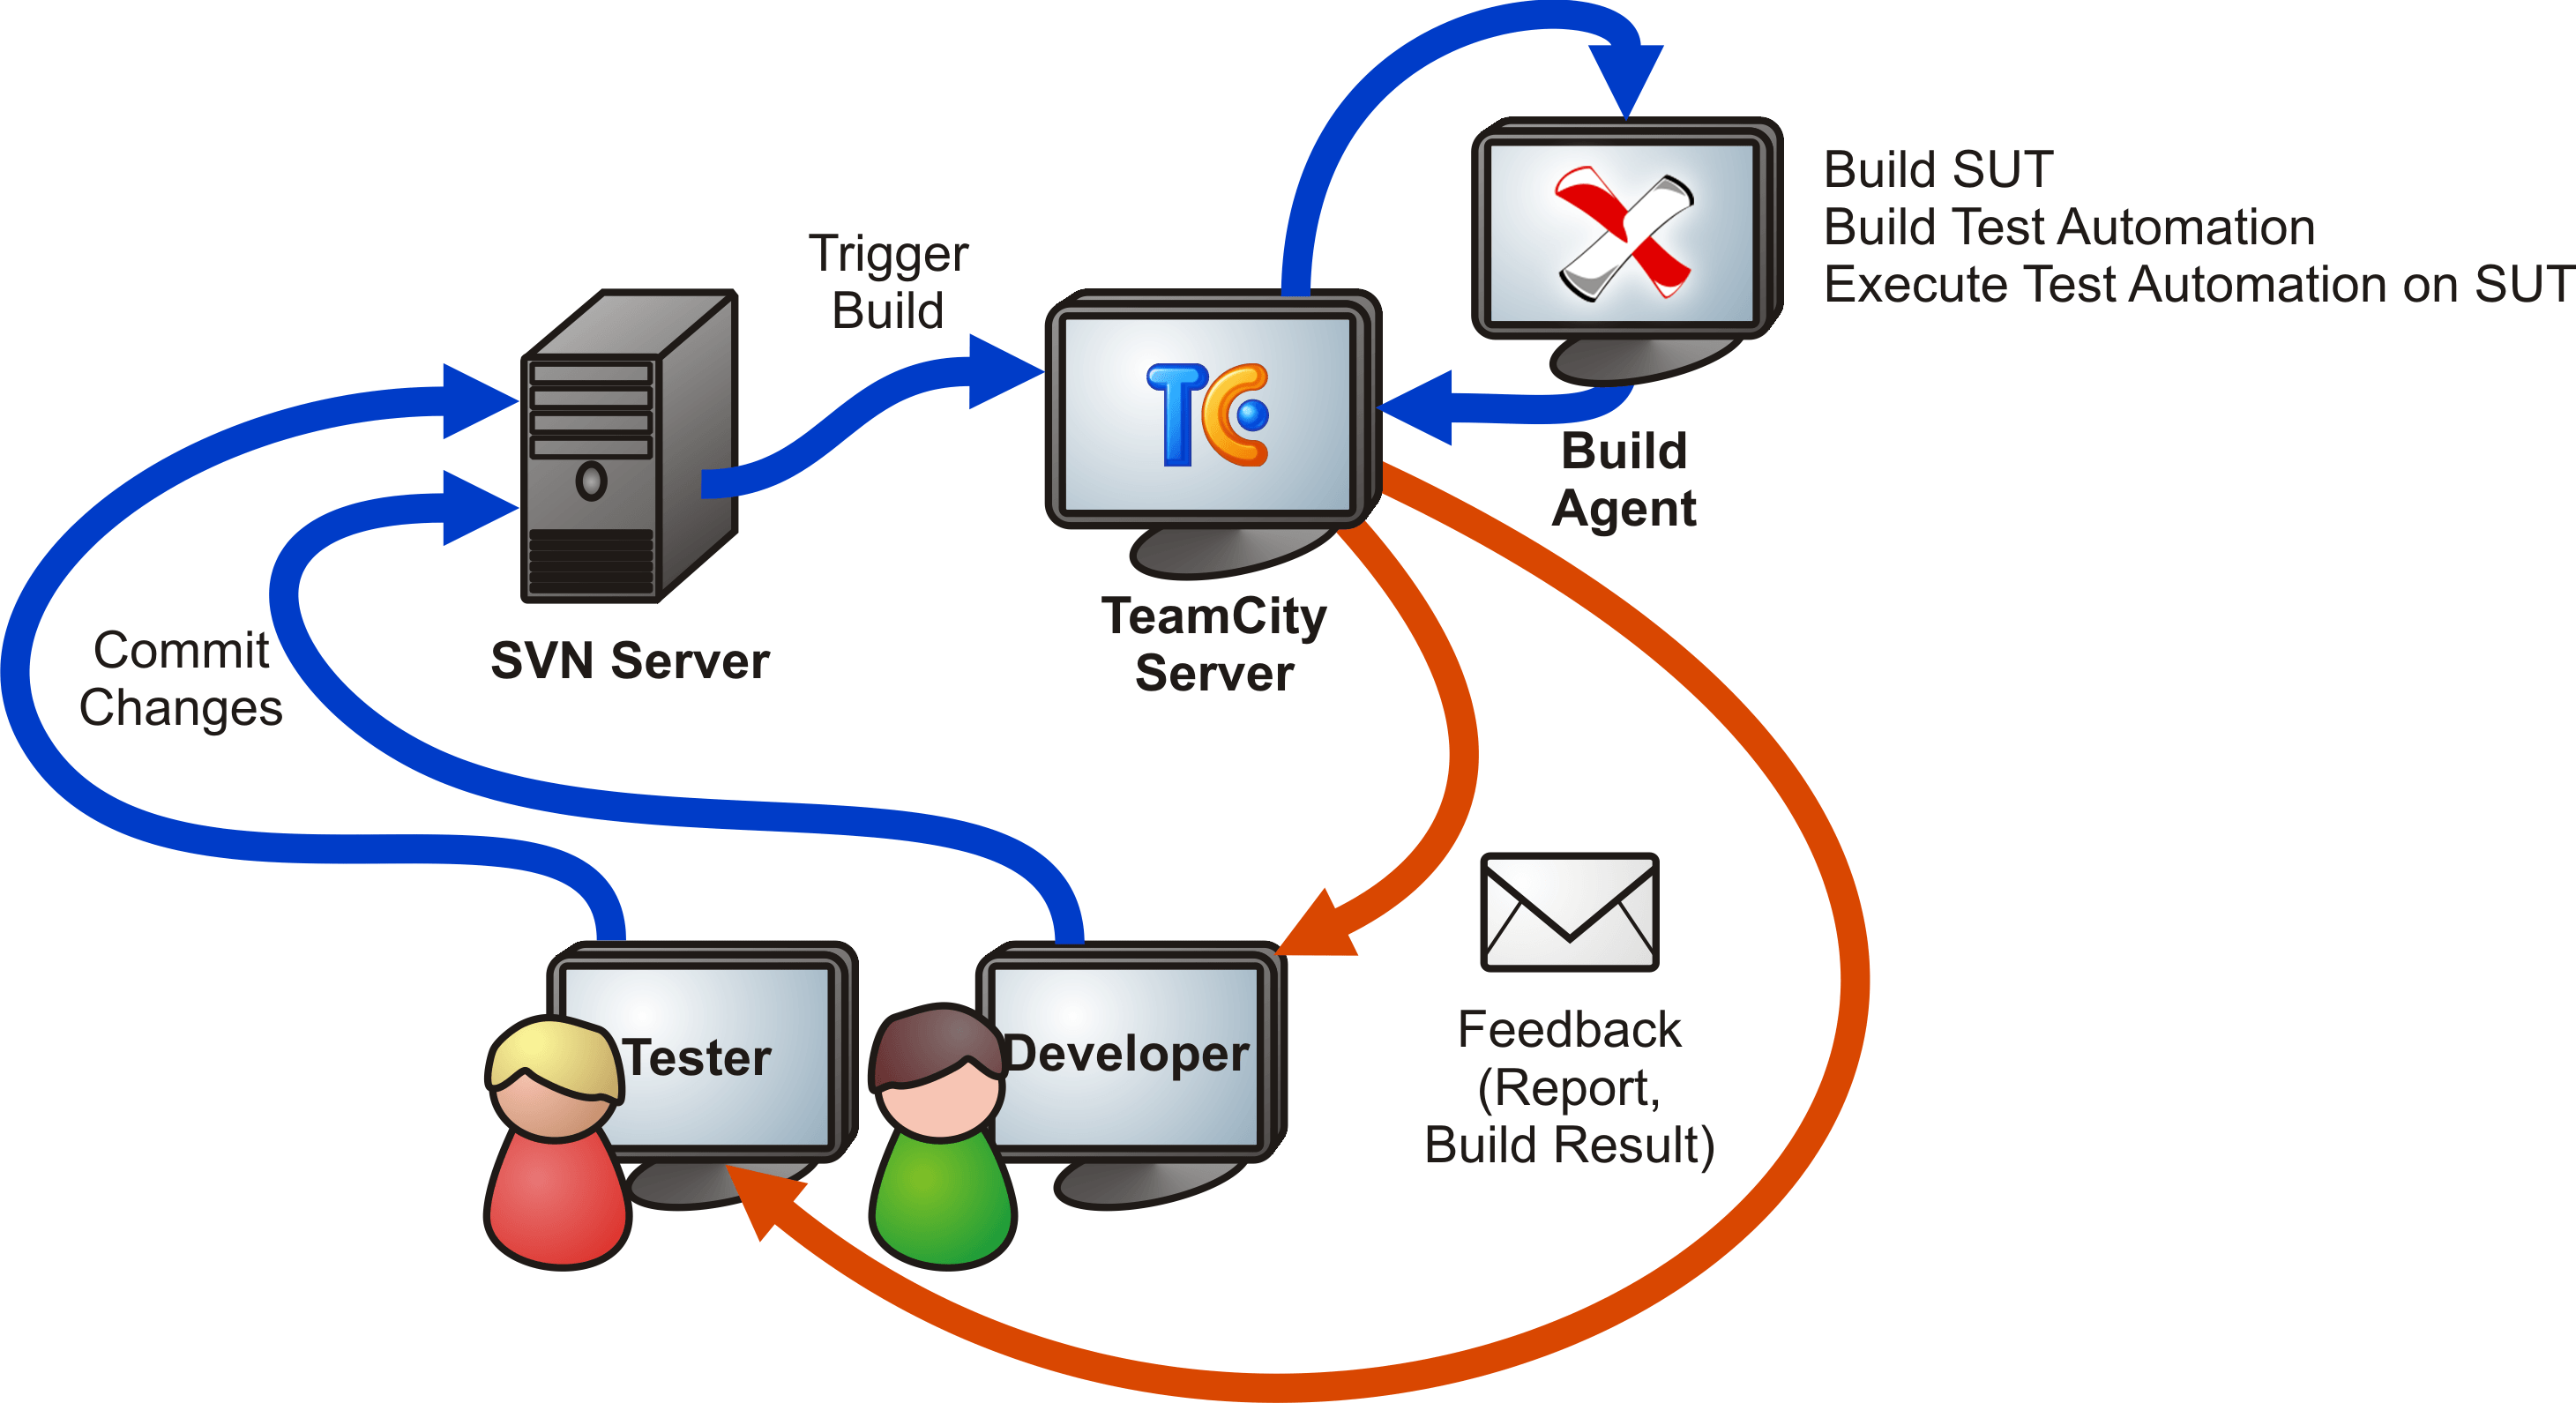
\includegraphics[width=\textwidth]{teamcity2}
\end{frame}
\lecturenotes
Архитектура TeamCity состоит из сервера интеграции, который управляет процессом, и <<фермы>> билд"---агентов, на которых и производится сборка и тестирование. Один агент может обрабатывать один проект, несколько агентов можно запускать параллельно
Важным моментом является то, что <<сервер интеграции>> и <<машина, на которой будет проходить этот процесс>>, "--- обычно (не обязательно) разные серверы. Более того, машин, на которых запускаются сборки и тесты, может быть несколько, даже много, и все на разных ОС.

~\cite{Habr_Team_City}

\begin{frame} \frametitle{TeamCity}
	\begin{block}{Общий сценарий на сервере будет выглядеть так:}
		\begin{itemize}
			\item Забрать свежие изменения из репозитория
			\item Скомпилировать проект
			\item Если всё прошло успешно на предыдущем шаге "--- прогнать юнит-тесты
			\item Если всё прошло успешно на предыдущем шаге "--- прогнать функциональные тесты
			\item Если всё прошло успешно на предыдущем шаге "--- залить изменения на тестовый сервер
		\end{itemize}
	\end{block}
\end{frame}

\lecturenotes

\begin{frame} \frametitle{Jenkins(Hudson)}
	
\includegraphics[width=\textwidth]{jenkins}
	\begin{block}{}
		Jenkins "--- проект для непрерывной интеграции с открытым исходным кодом, написанный на Java. Был ответвлён от проекта Hudson, принадлежащего компании Oracle. Распространяется под лицензией MIT
	\end{block}
\end{frame}

\lecturenotes
~\cite{Wiki_Jenkins}

\begin{frame} \frametitle{Jenkins (Hudson)}
	\begin{block}{Возможности}
		Может собирать проекты ApacheAnt и ApacheMaven(Java), а также исполнять shell\nobreakdash-скрипты и команды Windows \\
		Hudson имеет <<RemoteAccessAPI>>, позволяющее кроме прочего, инициировать сборку проекта, сделав GET\nobreakdash-запрос \\
		Поддерживает системы контроля версий:
		\begin{itemize}
			\item CVS
			\item Subversion
			\item Mercurial
			\item Git
			\item Clearcase и пр.
		\end{itemize}	
	\end{block}
\end{frame}
\lecturenotes
~\cite{Habr_Hudson}

\begin{frame} \frametitle{Jenkins (Hudson)}
	\begin{block}{Особенности}
		\begin{itemize}
			\item Архитектура Hudson'а построена на основе plugin'ов
			\item Сборка проекта заключается в запуске в определённом порядке установленных плагинов, включённых в настройках проекта
			\item Hudson позволяет изменять только порядок выполнения плагинов, входящих в группу <<сборка>> (порядок выполнения остальных плагинов в рамках своей группы определяется на основе значений аннотации @Execution коде плагинов)
		\end{itemize}
	\end{block}
\end{frame}

\lecturenotes
~\cite{Habr_Hudson}

\begin{frame} \frametitle{Jenkins (Hudson)}
	\begin{block}{Особенности}
		Плагины можно разделить на несколько условных групп, образующих цикл сборки:
		\begin{itemize}
			\item Управление исходным кодом (получение/обновление кода проекта из репозитория)
			\item Триггеры сборки (настройка времени автозапуска для сборки проекта)
			\item Среда сборки (настройка среды сборки проекта: версия JVM)
			\item Сборка (основной этап: запуск плагинов, осуществляющих логику сборки, интеграции и тестирования)
			\item Послесборочные операции (формирование/публикация отчётов, нотификация)
		\end{itemize}
	\end{block}


\end{frame}

\lecturenotes
~\cite{Habr_Hudson}

\begin{frame} \frametitle{Jenkins (Hudson)}
	\begin{block}{Особенности}
		По\nobreakdash-умолчанию Hudson поставляется с уже установленными плагинами для работы с SVN (централизованная система управления версиями) и Maven(инструмент для сборки java\nobreakdash-проектов) \\
		В случае если необходимо реализовать свой сценарий сборки, для которого не достаточно набора стандартных плагиновиз группы «Сборка», можно:
		\begin{itemize}
			\item Вызвать любой внешний исполняемый скрипт, реализующий этот сценарий (пункт ”ExecuteShell” из меню ”Addbuildstep”)
			\item Подключить плагин системы сборки проекта (Phing, Ant, Maven) и указать необходимую цель
			\item Написать свой плагин
		\end{itemize}
	\end{block}
\end{frame}

\lecturenotes
~\cite{Habr_Hudson}

\begin{thebibliography}{99}
\bibitem{Wiki_Build_automation} \href{https://en.wikipedia.org/wiki/Build_automation}
\bibitem{Habr_make} \href{https://habrahabr.ru/post/211751/}
\bibitem{Wiki_Apache_Ant} \href{https://ru.wikipedia.org/wiki/Apache_Ant}
\bibitem{Wiki_Apache_Maven} \href{https://ru.wikipedia.org/wiki/Apache_Maven}
\bibitem{Wiki_Gradle} \href{https://ru.wikipedia.org/wiki/Gradle}
\bibitem{Habr_Gradle} \href{https://habrahabr.ru/post/225189/}
\bibitem{Wiki_Continuous_integration} \href{https://en.wikipedia.org/wiki/Continuous_integration}
\bibitem{Habr_Team_City} \href{https://habrahabr.ru/company/skbkontur/blog/205402/}
\bibitem{Wiki_Jenkins} \href{https://en.wikipedia.org/wiki/Jenkins_(software)}
\bibitem{Habr_Hudson} \href{https://habrahabr.ru/post/108928/}
\bibitem{Custis_Continuous Integration} \href{http://lib.custis.ru/%D0%9D%D0%B5%D0%BF%D1%80%D0%B5%D1%80%D1%8B%D0%B2%D0%BD%D0%B0%D1%8F_%D0%B8%D0%BD%D1%82%D0%B5%D0%B3%D1%80%D0%B0%D1%86%D0%B8%D1%8F}
\bibitem{Yandex_Build_Automation} \href{https://events.yandex.ru/lib/talks/2709/}

\end{thebibliography}

\end{document}

%%% Local Variables: 
%%% mode: TeX-pdf
%%% TeX-master: t
%%% End: 
